% This is LLNCS.DEM the demonstration file of
% the LaTeX macro package from Springer-Verlag
% for Lecture Notes in Computer Science,
% version 2.4 for LaTeX2e as of 16. April 2010
%
\documentclass{llncs}
\usepackage{graphicx}
%
\begin{document}
%
\title{Mobile Application Development with MELON}
%
\author{Justin Collins \and Rajive Bagrodia}
%
%%%% list of authors for the TOC (use if author list has to be modified)
\tocauthor{Justin Collins, Rajive Bagrodia}
%
\institute{University of California Los Angeles, Los Angeles CA, USA,\\
\email{\{collins, rajive\}@cs.ucla.edu}}

\maketitle              % typeset the title of the contribution

\begin{abstract}
The abstract should summarize the contents of the paper
using at least 70 and at most 150 words. It will be set in 9-point
font size and be inset 1.0 cm from the right and left margins.
There will be two blank lines before and after the Abstract. \dots
\keywords{computational geometry, graph theory, Hamilton cycles}
\end{abstract}
%
\section{MELON Design}\label{sec:design}

The design of MELON is centered around a distributed shared message store. Each device in the network may host any number of applications which access and contribute to the shared message store. Each application hosts a local message store which may be accessed by any other local or remote application. Applications request messages (which may be local or remote) using message templates.

By communicating through a shared message store, the concept of connections between hosts is eliminated and thus disconnections are no longer an application layer concern. Hosts suddenly leaving the network does not disrupt an application and applications do not need to handle operations failing from intermittent network connectivity or physical wireless interference. The application is insulated from these issues by the semantics of the operations.

Messages are sent and received asynchronously by storing and retrieving them from the shared message store, removing the need for a persistent connection. This provides temporal decoupling between hosts, since messages can still be delivered even after prolonged disconnections.

The dynamic network topology of MANETs creates a challenge which maintaining any type of logical or overlay network, so MELON does not rely on a particular network structure. Discovery of available messages is performed on-demand for each operation. While this does increase the amount of communication required for each operation, it avoids global state and allows the network to change at any time.

MELON also provides spatial decoupling by matching messages based on content, instead of a host address or location. The messages themselves may physically reside on any host in the network. The sender of a message is not aware of the receivers' identities nor even how many receivers might read a message. This frees applications from tracking remote addresses or contacting a directory service to find remote resources.

The shared wireless communication medium in MANETs is well-suited to multicast communications. MELON supports multicast communication by allowing any number of receivers to read the same message. MELON also provides bulk receives, which allow applications to efficiently receive multiple messages from multiple hosts in a single operation.

Applications often also require unicast communication. While unicast communication can be accomplished by storing regular messages in MELON, these can be disrupted by a process removing a message intended for a different receiver. It is also possible to eavesdrop on messages by reading but not removing a message. For applications such as instant messaging, it is important to have private unicast communication. In MELON, messages may be directed to a specific receiver to ensure the messages are only taken by the intended recipient.

MELON also includes features uncommon to shared message stores to further simplify application development in MANETs. First, messages are returned in first-in first-out order per host. When a host receives a message request, it returns the oldest matching message in its local storage. In applications where a single host generates the majority of the messages, this eliminates the need to order messages on the receiver side. 

Secondly, MELON provides operations to only read messages which were not previously read by the same process. This enables an application to read all matching messages currently in the message store, then read only newly-added messages in subsequent operations. It also prevents an application from reading the same message twice.

Finally, MELON differentiates between messages intended to persist and be read by many receivers versus messages expected to be removed from the message store. For example, messages in a news feed would have many readers but messages should not be removed. In contrast, in a job queue each job should be removed by exactly one worker. MELON provides operations to support both scenarios.

\subsection{MELON Operations Overview}

Messages can be copied to the shared message store via a \textbf{store} or \textbf{write} operation. A \textbf{store} operation allows the message to later be removed from the storage space. Messages saved with a \textbf{write} operation cannot be explicitly removed from the storage space, only copied.

Messages added via \textbf{store} may be retrieved by a \textbf{take} operation using a message template which specifies the content of the message to be returned. A \textbf{take} operation will remove a message with matching content from the message store and return it to the requesting process. \textbf{take} operations are atomic: a message may only ever be returned by a single \textbf{take} operation.

A \textbf{read} operation will also return a message matching a given template, but does not remove the original message from the shared storage. Any number of processes may read the same message. However, repeated applications of a \textbf{read} operation in the same process will never return the same message. Only messages stored with \textbf{write} can be returned by a \textbf{read} operation.

The basic \textbf{take} and \textbf{read} operations return a single message per invocation. To facilitate the exchange of multiple messages, MELON includes the bulk operations \textbf{take\_all} and \textbf{read\_all}. The bulk versions operate the same as the basic operations, except all available matching messages will be returned instead of a single message. For \textbf{read\_all}, only messages which were not previously returned by a \textbf{read} or \textbf{read\_all} in the same process will be returned.

By default \textbf{take}, \textbf{take\_all}, \textbf{read}, and \textbf{read\_all} will block the process until a matching message is available. MELON also provides non-blocking versions of these operations. The non-blocking operations will return a null value if no matching messages can be found.

When a message is saved with a \textbf{store} operation, it may optionally be directed to a specific receiver. In a directed message, the identity of a receiver is included in the message as the addressee. Only the addressee may access a directed message through a \textbf{take}.

Due to the limited resources of most devices in a mobile network, storage space in MELON is explicitly bounded. Any message may be garbage collected prior to being removed by a \textbf{take} if capacity is reached.

\subsection{Operation Details}

Processes in MELON communicate by storing messages to a distributed shared message store and retrieving the messages based on templates. In this paper, we assume messages consist of an ordered list of typed values and optionally an addressee. However, nothing in the paradigm itself limits how messages might be constructed (e.g., they could be an unordered tuple with named values instead).

A message template is similar to a message, except it may contain both values and types. For example, a message containing \texttt{[1, "hello"]} could be matched by a template containing \texttt{[1, String]} or \texttt{[Integer, "hello"]} or \texttt{[Integer, String]}. A type will also match any subtypes.

Each operation is implemented as a separate function call. \textbf{store} and \textbf{write} operations have null return values and return as soon as the saved message is available in the message store. \textbf{take} and \textbf{read} operations block by default until a matching message is returned, but may be set to non-blocking on a per-call basis.

\begin{table}
\centering
\begin{tabular}{|c|c|c|}
\hline
\textbf{Operation} & \textbf{Return Type} & \textbf{Action} \\ \hline
\textbf{store}(\textit{message}, \textit{[address]}) & \textit{null} & Store removable message \\ \hline
\textbf{write}(\textit{message}) & \textit{null} & Store read-only message \\ \hline
\textbf{take}(\textit{template}, \textit{[block = true]}) & \textit{message} or \textit{null} & Remove and return message \\ \hline
\textbf{read}(\textit{template}, \textit{[block = true]}) & \textit{message} or \textit{null} & Copy and return read-only message \\ \hline
\textbf{take\_all}(\textit{template}, \textit{[block = true]}) & \textit{array} & Bulk remove messages \\ \hline
\textbf{read\_all}(\textit{template}, \textit{[block = true]}) & \textit{array} & Bulk copy read-only messages \\ \hline
\end{tabular}
\caption{MELON Operations}
\end{table}

When called, \textbf{store} saves a copy of the message in the message store. Messages saved with \textbf{store} may only be retrieved with a \textbf{take} or \textbf{take\_all} operation. If an address is provided, then only the host with a matching identity can remove the message.

The \textbf{write} operation also stores a single message in the message store, but the message may only be copied from the storage space with a \textbf{read} operation, never explicitly removed. Messages written with the \textbf{write} operation may be automatically garbage collected.

A \textbf{take} operation requires a message template as the first argument and an optional boolean for the second argument. The message template is matched against available messages in the message store which were added with a \textbf{store} operation. If a matching message is found, it will be removed from the message store and returned. Once a message has been returned by a \textbf{take} operation, it is removed from the message store and may not be returned by a subsequent operation in any process.

The \textbf{read} operation will only return messages stored with a \textbf{write} operation which have not already been read by the current process. If a message matching the given message template is available, it will be copied and returned, but not removed from the message store. Once a message has been returned to a process, the message is considered to have been read by that process and will not be returned by any subsequent \textbf{read} or \textbf{read\_all} operations in that process. A message may be \textbf{read} by any number of processes, but only once per process.

\begin{table}
\centering
\caption{Read from multiple processes}
\begin{tabular}{|c|c|c|} \hline
\textbf{Process A} & \textbf{Process B} & \textbf{Process C} \\ \hline
\texttt{write([1, "hello"])} & \texttt{m = read([Integer, String])} & \texttt{m = read([Integer, String])} \\ \hline
\end{tabular}
\label{fig:readprocesses}
\end{table}

Table \ref{fig:readprocesses} illustrates one process writing a single message containing the integer \texttt{1} and the string \texttt{"hello"}. Processes B and C each perform a \textbf{read} operation with the template which matches the message stored by process A. Since \textbf{read} does not modify the storage space, the value of \textit{m} for both process B and C will be a copy of the message \texttt{[1, "hello"]} from process A.

The \textbf{take\_all} and \textbf{read\_all} operations are used to retrieve a group of matching messages instead of a single message. Otherwise, the semantics match \textbf{take} and \textbf{read}: \textbf{take\_all} can only remove messages from \textbf{store} operations, and \textbf{read\_all} only returns unread messages from \textbf{write} operations.

\begin{table}
\centering
\caption{News server and reader}
\begin{tabular}{|c|c|} \hline
\textbf{News Server} & \textbf{News Reader} \\ \hline
\begin{minipage}{2.45in}
\begin{verbatim}

function report(category, headline) {
   write([category, headline])
} 
\end{verbatim}
\end{minipage}
&
\begin{minipage}{2.5in}
\begin{verbatim}


function fetch(category) {
   return read_all([category, String])
}
\end{verbatim}
\end{minipage}
\\ \hline
\end{tabular}
\label{fig:newsreader}
\end{table}

Table \ref{fig:newsreader} demonstrates a use of \textbf{read\_all}. One or more processes generate news messages containing a news category and headline. To ensure all interested parties can read the news, the server uses \textbf{write} to disallow a reader from removing a news item and preventing other readers from reading it. Any number of processes can consume the news as readers. The \texttt{fetch} method in Table \ref{fig:readprocesses} uses \textbf{read\_all} to return all news items in a given category. Repeated calls to \texttt{fetch} will only return news items not previously seen.

By default, all retrieval operations will block the application until at least one matching message is found. The operations can also be performed in nonblocking mode, in which case \textbf{take} and \textbf{read} return null when no matching message is found, while \textbf{take\_all} and \textbf{read\_all} return empty collections.
   
\section{MELON Implementation}\label{sec:implementation}

\begin{figure}
\centering
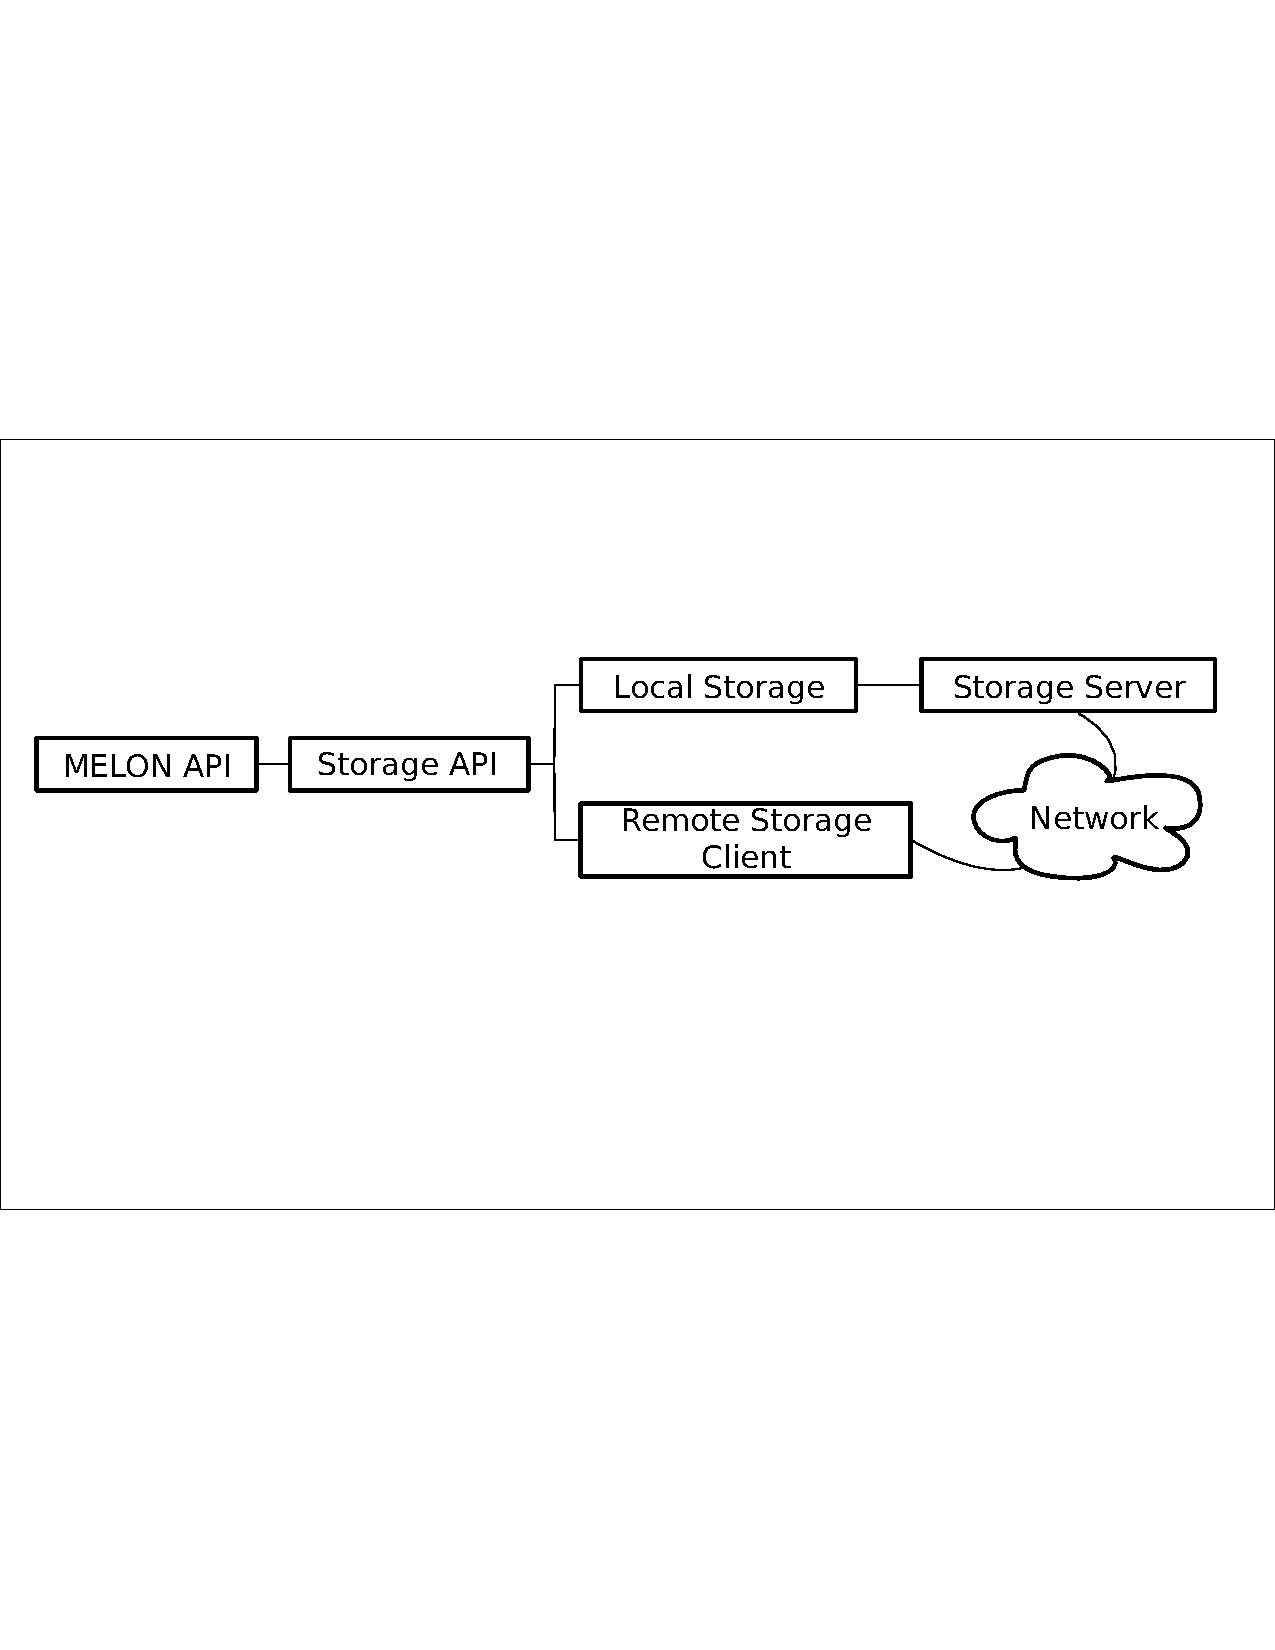
\includegraphics[scale = .50, clip, trim = 10px 350px 10px 312px]{figures/paradigm_arch.pdf}
\caption{Paradigm Architecture}
\label{fig:architecture}
\end{figure}

We developed a prototype implementation of MELON to validate our design and obtain empirical performance data. The architecture illustrated in Figure \ref{fig:architecture} is split into five parts. The MELON API is the only interface exposed to the application and provides the six operations described above. The MELON API interacts with the distributed message storage through the storage API, which provides the same interface for both local and remote storage. The storage server proves a network interface to a local storage space and accepts connections made through the remote storage stub.

Local storage is implemented as two dynamic arrays, one for \textbf{write}/\textbf{read} messages and the other for \textbf{store}/\textbf{take} messages. For atomic updates, the \textbf{write}/\textbf{read} array uses a readers/writer lock to allow multiple \textbf{read} operations to access the array in parallel, but locks the array for \textbf{write} operations. The \textbf{store}/\textbf{take} array does not permit concurrent operations, as \textbf{store} and \textbf{take} modify the store. The two arrays may be accessed and modified independently.

Network communication is handled using ZeroMQ\cite{hintjens2013zeromq}, a high performance networking library. For the prototype, the networking was intentionally kept simple. For example, a \textbf{read} request queries remote hosts in random order and stops when a matching result is returned. This could possibly be improved using multicast, it would complicate the implementation by requiring the client to handle multiple asynchronous responses, select one, request the actual message, and handle failure scenarios if the matching message cannot be returned. We trade potential performance gains for simplicity. 

For \textbf{read} and \textbf{read\_all} operations, it is necessary to track which messages have been read. Each process maintains its own list of read messages, which it sends with each \textbf{read} request. We use a compact sparse bit set to transfer this information efficiently. We measure this overhead in Section \ref{sec:overhead}.


\subsection{Tracking Read Messages}\label{sec:readmessages}

    When a messages is stored, it is given a unique identifier [\textit{P}, \textit{M}], where \textit{P} is a globally unique integer identifier for the storing process, and \textit{M} is an integer identifier for the stored message. Each process maintains an integer ID which is incremented for each store. Messages stored from the same process with sequential \textbf{store} or \textbf{write} operations will have consecutive \textit{M} values and share the same \textit{P} value.

    In order to prevent \textbf{read} from returning a message more than once in the same process, each process maintains a sparse bit set for each process from which a message has been read. The identifier [\textit{P}, \textit{M}] is condensed into a single unique integer \textit{Q} using the ``elegant pairing function''\cite{szudzikelegant} shown in Equation \ref{eq:elegantpairing}. Since the values of \textit{Q} will be consecutive integers for all consecutive values of $M < P$, it is helpful to set \textit{P} to be higher than the number of expected messages. The value \textit{Q} is then stored in a sparse bit set with a hash table using integer keys and bit field values.

 \begin{equation}
   f(M,P) = \left\{
     \begin{array}{lr}
       M^{2} + M + P & : M \geq P \\
       P^{2} + M & : M < P
     \end{array}
   \right.
   \label{eq:elegantpairing}
\end{equation}

The index \textit{i} in the sparse bit set indicates the range stored in the bit set. If \textit{w} is the number of bits for each bit set, then each bit field can store up to \textit{w} values of \textit{n}, where $w \times i \leq n < w \times (i + 1)$. A message with ID \textit{n} will be stored in index $n/w$ by setting the bit at $n \bmod w$ in the bit field to \texttt{1}.

If the index value is of size \textit{l} bits and the bit field contains \textit{w} bits, then the cost for storing a single value is $l + w$. For storing a set of consecutive values of length \textit{m}, the cost is $\lfloor \frac{m \times l}{w} \rfloor + m$ bits. In other words, the total cost is one bit per message, plus the cost of one index per \textit{w} messages.

%
%\begin{table}
%\centering
%\caption{Sparse bit set example}
%\begin{tabular}{|c|c|} \hline
%Index & Bit Field \\ \hline
%0 & 01100001 \\ \hline
%4 & 00010000 \\ \hline
%15 & 10100100 \\ \hline
%\end{tabular}
%\label{fig:bitset}
%\end{table}

Consecutive messages (from any starting value) are the best-case scenario for sparse bit sets. In the worst case, the message IDs differ by at least \textit{w}, causing each message to incur a $l + w$ cost for storage and a total cost of $m \times (l + w)$ bits.

Determining if a message [\textit{P}, \textit{M}] is in the set is accomplished by first computing \textit{Q}. If there is no key at index $Q/w$, the message has not been read. Otherwise, retrieve the bit field \textit{b} at index $M / w$. If $b \wedge 2^{M \bmod w} \neq 0$ then the message has been read, otherwise the message is unread.
    
\subsection{Retrieving Unread Messages}

When performing a \textbf{read} or \textbf{read\_all} operation, MELON must only return messages which have not previously been returned by a \textbf{read} or \textbf{read\_all} to the requesting process. Since every process has its own set of of messages which it has read, the requesting process sends this set of read messages to the requestee.

A \textbf{read} request contains a message template and the set of messages which have already been read. The receiving process will match the message template against the messages in its local storage, excluding messages which are in the set of read messages. If a matching unread message is found, the process will send the message to the requestor. If multiple matching unread messages are found, the process will send the message with the lowest message ID. If no matching messages are found, the process returns an empty response.

Similarly, \textbf{read\_all} requests also include the message template and the set of read messages. A process receiving a \textbf{read\_all} request will match the message template against messages in the local storage, excluding messages in the set of read messages. The process will then return all matching unread messages to the requestor. If no matching unread messages are found, the process returns an empty set.

\section{Related Work}\label{sec:relatedwork}

The concept of a distributed shared message store is based on the idea of tuple spaces introduced with the Linda\cite{linda} coordination language. Several projects have adapted tuple spaces to MANETs, including LIME\cite{lime}, MESHmdl\cite{meshmdl}, TOTA\cite{tota}, and EgoSpaces\cite{egospaces}, of which LIME is likely the most well-cited example.

The original version of LIME relies on explicit join and leave operations to federate distributed tuple spaces, which is at odds with the frequently unexpected disconnections in MANETs. \cite{limerevisted} discusses the difficulties LIME encounters when attempting to implement tuple space semantics, including situations that can lead to livelocks. LIME II\cite{lime2}, Limone\cite{limone}, and CoreLIME\cite{corelime} are projects intended to address the shortcomings in the original LIME.

REDS\cite{reds} and GREEN\cite{green} are examples of publish/subscribe adapted to MANETS. AmbientTalk\cite{ambienttalk} is an entire language for MANETs based on RPC and actors. Further surveys of middleware, languages, and communication paradigms for MANET development can be found in \cite{mine} and \cite{mwtrends}.

\subsection{Comparison to Existing Paradigms}

This section compares MELON to publish/subscribe, remote procedure calls (RPC), and tuple spaces: three distributed computing paradigms often used as the basis for MANET middleware.

\subsubsection{Disconnection Handling}

In the unreliable MANET environment, disconnections frequently occur during the exchange of messages. Since disconnections can be prolonged, the networking layers will assume the connection is entirely lost and cease retrying. By having a message persist in some way, a paradigm can overcome these disconnections and deliver the message at a later time.

Publish/subscribe allows message publication without any consideration for the state of the subscribers. Publish/subscribe itself does not specify how ``missed'' publications should be handled. A publish/subscribe system can utilize ``brokers'' which manage subscriptions and facilitate delivery of publications. Brokers can then serve as message buffers and provide more reliable message delivery in the face of disconnections. In distributed publish/subscribe systems, however, the brokers must be self-organizing, and in MANET this is complicated by how quickly the network can change. It is common for distributed publish/subscribe systems not to provide message persistence. If a subscriber is not available at the time of publication, the message will not be received.

Since RPC requires a connection for communication, disconnections typically cause RPC to block a process entirely until a remote node hosting an appropriate method is available. Messages themselves only exist briefly during the RPC transaction. Messages cannot be sent if a connection cannot be made to a remote host.
    
In tuple spaces and MELON, message persistence is inherent in the paradigms. In both paradigms, exchange of messages is achieved by storing the messages in a shared storage space. Any amount of time may elapse between the storage of a message and its retrieval. This allows reliable communication even in the face of prolonged disconnections and is the reason we have chosen it for MELON.

\subsubsection{Addressing and Discovery}

All of the paradigms discussed here provide indirect addressing of resources separated from the physical machines. Publish/subscribe uses topics or content to deliver message to subscribers, RPC uses class and method names, and tuple spaces and MELON retrieve messages by matching content to templates. While all three traditional paradigms originally relied on centralized services (brokers from publish/subscribe, service directories for RPC, and a centralized database for tuple spaces), simple distributed versions may be implemented by having each node act as part of a distributed service.
    
\subsubsection{Flexible Communication}

A general purpose communication paradigm for MANET applications should have the flexibility to support both unicast and multicast communication.

Publications in publish/subscribe are inherently multicast, since any number of nodes can subscribe. Unicast communication is much less comfortable in publish/subscribe, as it involves negotiating which topics should be used to identify which nodes. Publish/subscribe also does not provide any mechanism for ensuring or even acknowledging message delivery to any given subscriber, especially since publishers and subscribers are intended to be unaware of each other.

Since RPC mimics local method calls, it is natural that RPC is best suited for unicast communication, in which the message is the argument to the method and the return value is the response from the remote host. Assuming multicast RPC functions in the same manner, then a multicast RPC invocation would expect multiple return values, one from each remote host. In a MANET, it is likely not every remote host would reliably return a response, further complicating the semantics. A typical RPC invocation would block waiting for a response, but it is not practical to wait for all responses to a multicast RPC invocation when some responses may never be received. The use of futures or asynchronous callbacks can improve the situation, but causes semantics to differ even more from unicast RPC.

Tuple spaces are naturally multicast, since any number of nodes may read a given tuple. Unicast communication can be achieved by using a field in the tuple as the recipient’s address. The recipient then performs in operations on tuples with their address in order to receive the tuples.

MELON divides communications into three types: messages which can be received by any single recipient, messages which can be received by a specific single recipient, and messages which can be received by any number of recipients. Messages sent with a store operation can only be consumed by a single take operation. Directed messages are also sent with store, but can only be consumed with a take performed by the intended recipient. write stores messages which may be read by any number of recipients and can never be removed by a take. MELON also provides the ability to receive multiple messages at once with \textbf{take\_all} and \textbf{read\_all} operations.
    
Networked applications also commonly require private, unicast communication. For example: SMS services, direct messaging in social networks, or communication of sensitive data. For our purposes, private communication is the exchange of messages between two parties which cannot be disrupted or eavesdropped upon by a third party from within the context of the paradigm itself. In other words, concerns such as encrypting data or sniffing network traffic would be outside the paradigm context.

RPC is unicast by default and there is no method in the paradigm for eavesdropping or disrupting RPC between two nodes. However, RPC has a different complication: remote hosts are generally identified by their exposed methods and there is no mechanism for attaching identity to the hosts. RPC will connect to any remote method with the expected API. So while private communication is the default in RPC, there is an addressing issue which makes it complicated to communicate with a specific recipient.

Communication in publish/subscribe is public and multicast by nature. Any subscriber can subscribe to any set of publications, making it simple to eavesdrop on communications. Bidirectional communication is also difficult in publish/subscribe, since there is no information attached to a publication indicating the identity of the publisher. This is by design, but it complicates situations in which two hosts need to dialog.

In tuple spaces, tuples are public and available to any recipient. Not only can any node read any communications without detection, any node can also disrupt communications by removing tuples intended for a specific recipient.

MELON provides two access control mechanisms for messages. First, messages are explicitly either available for any recipient to remove or limited to read-only operations. Read-only messages are useful in scenarios where information is intended to be widely available and removal of the information would be considered disruptive to the application. Second, if messages are directed to a specific recipient, then the paradigm implementation is responsible for disallowing any other nodes from reading or removing the given message. This allows simple private unicast communication between nodes.

\subsubsection{Multiple Read Problem}

The multiple read problem \cite{mrdp} is specific to tuple spaces: in a situation where the tuple space contains many tuples of interest, how do multiple readers read \textit{all} relevant tuples? In tuple spaces, the non-destructive \textbf{rd} operation returns a copy of a matching tuple, but it may return the same tuple any number of times since the tuple is chosen nondeterministically between all matching tuples. In many tuple space implementations, this occurs because the tuples are stored sequentially and so the first matching tuple is always the same\cite{de2012new}.

One solution is to use a single tuple as a mutex, lock the tuple space, remove all matching tuples with \textbf{in}, then replace them in the tuple space. However, this ruins any concurrency the tuple space could have had with multiple readers.

Another solution is to provide a bulk \textbf{rd} operation to return all matching tuples. However, once a ``snapshot'' of the tuple space has been taken with a bulk \textbf{rd}, new matching tuples may be introduced. A second bulk \textbf{rd} would return both the old (already seen) tuples and the new tuples. A similar suggestion from \cite{edwards2001jini} is to remove all matching tuples inside a transaction, then abort the transaction in order to actually leave the tuple space unmodified. However, this again leaves the problem of separating new tuples from previously-read tuples.

MELON avoids this issue by only returning messages unread by the current process. Assuming a fixed set of stored messages, repeated \textbf{read} operations in the same process would eventually return each matching message exactly once. MELON also provides the \textbf{read\_all} operation for reading messages in bulk. Unlike the tuple space version, \textbf{read\_all} only returns unread messages. This allows applications to easily read all existing matching messages, after which \textbf{read\_all} will only return messages stored since or unavailable during the previous operation.


\bibliographystyle{unsrt}
\bibliography{refs}

\end{document}
